\documentclass[a4paper,twoside]{article}

\usepackage{epsfig}
\usepackage{subfigure}
\usepackage{calc}
\usepackage{amssymb}
\usepackage{amstext}
\usepackage{amsmath}
\usepackage{amsthm}
\usepackage{multicol}
\usepackage{pslatex}
\usepackage{apalike}
\usepackage{SCITEPRESS}
\usepackage[small]{caption}

%%% For charts%%
\usepackage{tikz}

\subfigtopskip=0pt
\subfigcapskip=0pt
\subfigbottomskip=0pt

\begin{document}

\title{From simulation to development in MAS: A JADE-based Approach}

%\author{\authorname{João P. C. Lopes\sup{1} and Henrique Lopes Cardoso\sup{1}}
%	\affiliation{
%		\sup{1}LIACC,
%		Faculty of Engineering of University of Porto,
%		Rua Dr. Roberto Frias, Porto, Portugal
%	}
%	\email{\{lopes.joao.pedro, hlc\}@fe.up.pt}
%}

\keywords{MAS, MABS, Framework Integration}

\abstract{Multi-agent systems (MAS) present an interesting approach to the efficient development of modular systems. Frameworks exist that aid the development of this class of systems but, most of the time, no single one serves a project fully. Some works propose the integration of frameworks with other frameworks or with custom adapters to complement most of their missing features. This paper proposes the use of JADE as a MAS development environment and the use of simulation frameworks like Repast as the engine for developing JADE-based simulations. Repast is extended with and API called SAJaS, which implements a set of JADE features and allows the creation of simulations using a complex agent infrastructure. A conversion tool called MASSim2Dev bridges the gap between MAS development and simulation by mapping SAJaS's and JADE's API. This solution provides increased simulation performance while enabling programmers to quickly get started with development or simulation of their multi-agent models. Validation tests show how using MASSim2Dev preserves the original functionality of the system.}

\onecolumn \maketitle \normalsize \vfill

\section{\uppercase{Introduction}}
\label{sec:introduction}

\noindent Multi-agent systems (MAS) present an interesting approach to the efficient development of modular systems, composed by autonomous, interacting computational units called agents. Frameworks exist that aid the development of this class of systems and they range from mostly general-purpose frameworks to domain-specific in an array of different domains. Multi-agent-based simulations (MABS) are a kind of agent applications with multiple purposes such as simulating urban traffic and social behaviour. Their execution is typically fast paced and are usually lexss complex in their implementation of agent and communication infrastructure.

\subsection{Motivation}
MABS are sometimes used on the course of the development of a full-featured MAS -- for instance, for testing purposes -- for the potential gains in performance when simulating MAS. 
However, most platforms for MAS development are not well suited for MABS development due to scalability limitations\cite{mengistu2008scalability}. Some related works were studied that demonstrate interest in solutions that make MABS more easy to be created using MAS development frameworks. Furthermore, an opportunity exists to partially automate the development of robust MAS from a previously tested simulation.

JADE \cite{bellifemine2007developing}, a very popular MAS development framework allows the creation of seamless distributed agent systems and complies with FIPA standards for agent interaction. Unfortunately, its multi-threaded architecture falls short in delivering the necessary performance to run a local simulation with a large number of agents.

Repast \cite{collier2003repast} is an agent-based simulation toolkit that allows creating simulations using rich GUI elements and real time agent statistics. It can easily handle large numbers of agents in a single simulation. Unlike JADE, though, Repast lacks much of the infrastructure for agent creation and interaction.

The main motivation for this paper lies in the potential performance gains when using agent simulation frameworks to produce a simulation of a MAS more complex than those typically developed with such frameworks. Some works \cite{garcia2011misia,gormer2011jrep} propose, as a solution for bridging the gap between MAS development and simulation, an integration of JADE and simulation features by extending this framework with a simulation layer created from scratch, or by integrating another framework, such as Repast.

\subsection{Goals}
This paper proposes the development of an integrated solution for bridging the domains of simulation and development of MAS. In order to do that, two main goals were identified.

\begin{enumerate}
  \item \textbf{First}, the creation of an adapter or API that would allow developers to abstract from simulation frameworks' features. It does so by reimplementing from scratch many JADE features, including its implementation of FIPA specifications for agent interaction and management. Since the API's architecture is very close to JADE's, conversion becomes more straightforward.
  \item \textbf{Second}, the development of a code conversion mechanism. By abstracting from the simulation tools and creating a MAS-like MABS, it becomes possible and more straightforward to engineer a tool that performs the automatic conversion of these MABS into equivalent MAS.
\end{enumerate}

This system is specially aimed at JADE developers who need to create a simulation of their already-developed MAS. By converting their code, the developer can perform tests and simulation and later convert the simulation back to a MAS, preserving all changes. JADE developers can also create simulations from scratch using frameworks like Repast using familiar JADE-like features, which would then be converted to a full features JADE MAS. Finally, this system is also of interest to Repast developers who desire to expand their knowledge of MAS development using more complex frameworks.


\section{\uppercase{Related Work}}
\label{sec:Background}
\noindent Several frameworks exist that offer support to the development of MAS or MABS. Some are domain specific, meaning that their purpose was well defined in their conception. MASeRaTi\cite{ahlbrecht2014scalable}, MATSim\cite{balmer2008agent} and SUMO\cite{SUMO2012} are some examples of MABS frameworks for traffic and transports simulation. 

Other works like Repast\cite{collier2003repast}, NetLogo\cite{tisue2004netlogo}, GALATEA\cite{davila2000galatea} and Plasma \cite{warden2010towards} are considered general-purpose. This list comprises only tools that are free and open source and is not meant to be exhaustive.

Some works propose approaches that are very similar to the solution proposed in this paper, namely the bridging of the domains of MAS and Simulation. MISIA, JRep and Plasma were built on top of JADE to create a simulation environment based on it. These three works were studied with more detail due to these similarities.

\subsection{MISIA}
MISIA is a middleware whose goal is to enhance the simulation of intelligent agents and to allow the visualization and analysis of agent's behaviour. It was developed by the Bioinformatic, Intelligent Systems and Educational Technology Research Group (BISITE) from Universidad de Salamanca\footnote{http://bisite.usal.es/}. It is no longer an active project; as a research experiment, work on this middleware evolved into other more specific tools.

MISIA's approach, as suggested by Figure \ref{fig:misia}, is to use a middle layer that acts as the bridge between two other layers that interact with JADE and Repast. By extending the agents in Repast and JADE, communicating through a coordinator and synchronizing their state, these agents work as a single one.

\begin{figure}
	\centering
	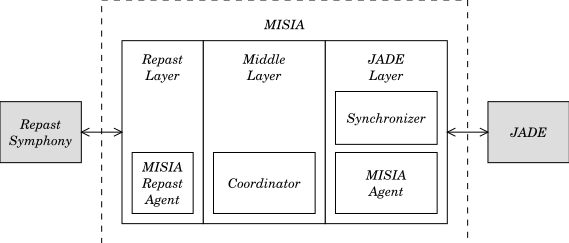
\includegraphics[width=\linewidth]{../figures/MISIA.pdf}
	\caption[MISIA's architecture]{High-level representation of MISIA's architecture (adapted from \cite{garcia2011misia})}
	\label{fig:misia}
\end{figure}

One of the challenges identified by the authors when re-implementing the FIPA interaction protocols was synchronizing them with the Repast tick-based simulation model. Given JADE's event-driven architecture, MISIA proposes the use of a coordinator agent that informs the JADE-Agent when a tick has passed. It also proposes its own implementation of the interaction protocols supported by JADE, making them tick-friendly.

\subsection{JRep}
JRep's approach is not as complex as MISIA's. By having the Repast Simphony agent encapsulate a JADE agent representation, synchronization is immediate and is assured without requiring an external coordinator.
The two agent representations take care of synchronizing any state changes.
Figure \ref{fig:jrep} represents the basic structure of JRep.

\begin{figure}
	\centering
	\includegraphics[width=\linewidth]{../figures/jrep.pdf}
	\caption[JRep's architecture]{High-level representation of JRep's architecture (adapted from \cite{gormer2011jrep})}
	\label{fig:jrep}
\end{figure}

Each agent takes care of interfacing their respective frameworks. The interaction between agents in JRep is performed using FIPA ACL and the protocol implementations are those provided by the JADE platform. Similarly to MISIA, an Agent Representation Interface is used to introduce the concept of schedule in the JADE agent.

\subsection{PlaSMA}
Unlike the two previous frameworks, the PlaSMA system is based solely on the JADE platform. The distributed simulation is synchronized by entities called ``Controllers'' who communicate with the ``Top Controller'', keeping the pace of the simulation and handling agent lifecycle management as well. Figure \ref{fig:plasma} illustrates this architecture. PlaSMA, unlike MISIA and JRep, is still an active project.

\begin{figure}
	\centering
	\includegraphics[width=\linewidth]{../figures/PlaSMA.pdf}
	\caption[PlaSMA's architecture]{High-level representation of PlaSMA's architecture (adapted from \cite{warden2010towards})}
	\label{fig:plasma}
\end{figure}

\subsection{Comparison}

JADE is a very rich platform but, for many simulation scenarios, the overhead it introduces has a significant impact on simulation performance \cite{mengistu2008scalability}.

Even though both MISIA and JRep attempt to integrate the features from both JADE and Repast, as far as Repast simulations are concerned JADE's multi-threaded infrastructure affects their performance very significantly. The main advantage of our approach is, therefore, the possibility of using Repast with JADE features, namely FIPA specifications including interaction protocols, without the need to interface with JADE. 

\section{\uppercase{Proposal}}
\label{sec:Proposal}
\noindent In order to benefit from different features, modelling the same system in multiple development environments is often necessary. The two main goals of this paper can be defined with two concrete solutions:

\begin{enumerate}
  \item The \textbf{Simple API for JADE-based Simulations (SAJaS)}, which provides a set of features present in JADE; those features were reimplemented from scratch in an attempt to simplify their internal complexity, preserving JADE-like external execution;
  \item The \textbf{MAS Simulation to Development code conversion tool (MASSim2Dev)} in the form of an Eclipse plug-in that is capable of mapping JADE and SAJaS features and convert applications developed using one into applications based on the other, automatically. The plugin has no Repast or JADE dependencies in the code, buts contains a dictionary file that is specific to JADE and Repast.
\end{enumerate}

SAJaS is an API meant to be used with simulation frameworks to enable JADE-based features in them, including agent interaction protocols and agent management services. It also uses JADE's concept of behaviours which encapsulate most of agents' actions.

SAJaS was initially created to be used with Repast Simphony but was developed to allow its integration with other simulation framework. To do so, SAJaS behaviours must be scheduled by the new framework a new agent implementation must be developed.

When developing SAJaS a close semblance to JADE's own API was kept, not only to make the code conversion more straightforward, but to allow proficient JADE developers to create SAJaS-based simulations using a familiar JADE-based API.
%MASSim2Dev was developed as an Eclipse plugin. It provides programmers with two possible actions: convert code from JADE to SAJaS and in the opposite direction.

SAJaS does not yet implement all JADE features. A set of the most common features were selected which allows for the simulation of scenarios with some complexity, including communication between agents and the creation of custom behaviours. Features in JADE applications which are not available in SAJaS will typically be shown as errors when converted; MASSim2Dev simply ignores them and they should be re-implemented manually as necessary.

\subsection{Usage Scenarios}
\label{sec:solution-scenarios}
%In this section, show how the whole setup is used with detailed use cases
Figure \ref{fig:prototypeFlow} illustrates the scenarios where this system is expected to be useful.

One possible scenario is when a JADE developer created a JADE MAS and desires to perform some tests and simulations in a local and controlled environment. The developer can use this tool to convert the MAS into a MABS. Eventually, the application can be converted back if changes were made while in the simulation format.

A second possible scenario could be that of a developer that intends to create a MABS with the goal of later creating a MAS out of it. This could be a Repast developer who desires to create more complex agent simulations or a JADE developer that wants to create Repast simulations using familiar JADE-like tools.

A third scenario is when a developer simply wants to create a complex agent-based, FIPA-compliant simulation. In this case, there is no need for a code conversion tool, but SAJaS can be used as a standalone library.

\begin{figure}
	\centering
	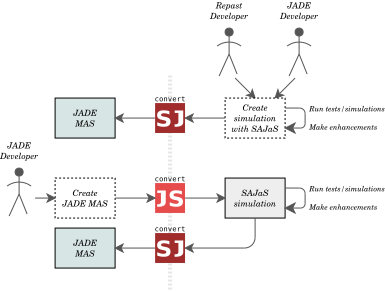
\includegraphics[width=\linewidth]{figures/prototypeFlow.pdf}
	\caption{
		Possible work flows for SAJaS users. ``SJ'' and ``JS'' represent conversion from SAJaS to JADE and the reverse, respectively.
	}
	\label{fig:prototypeFlow}
\end{figure}

\section{\uppercase{SAJaS}}
\label{sec:SAJaS}
\noindent From the point of view of the MAS programmer, working with this API feels the same as working with JADE, although limited to the presently available features. However, SAJaS has a much simpler internal architecture, which attempts to implement only the fundamental components needed for everything else to work. The most evident feature that was not ported from JADE was the network layer that enables the creation of distributed MAS.

The diagram in Figure \ref{fig:arch} represents a simplified version of SAJaS. The classes with doted border are internal and specific to SAJaS. All other classes are part of the API. The BehaviourAction and the RepastAgent offer support to Repast. More specifically, the BehaviourAction is responsible for interfacing Repast Symphony and scheduling the execution of all behaviours.

\begin{figure}[h]
	\centering
	\includegraphics[width=\linewidth]{figures/sajas_arch_simple.pdf}
	\caption{Simplified architecture of SAJaS}
	\label{fig:arch}
\end{figure}

Figure \ref{fig:arch_proto} shows the implementation of behaviours in SAJaS with more detail. The Behaviour superclass contains methods that are triggered by certain events.

\begin{enumerate}
	\item \texttt{action} is called once per tick
	\item \texttt{onStart} is called immediately before the first call to \texttt{action}
	\item \texttt{onEnd} is called right after the behaviour ended;
	\item \texttt{done} is called every tick to determine if the behaviour has ended and if true is returned, it triggers \texttt{onEnd}.
\end{enumerate}

\begin{figure}[h]
	\centering
	\includegraphics[width=\linewidth]{figures/sajas_arch_proto_simple.pdf}
	\caption{SAJaS's behaviour implementation}
	\label{fig:arch_proto}
\end{figure}

The methods \texttt{action} and \texttt{done} are abstract in Behaviour, so  other behaviours have to implement it. Methods \texttt{onStart} and \texttt{onEnd}, though, are implemented but do nothing in Behaviour.

The five ``responder'' and ``initiator'' classes implement the two protocols currently available in SAJaS. The FSMBehaviour, which they extend, contains a dynamic list of states and transitions. These can be registered and unregistered at runtime, typically before initiating the behaviour or in its setup. Each state is itself a behaviour.

Each protocol can be represented as a different state machine. For instance, in a Contract Net, the initiator's state starts as ``sending CFP'', then ``waiting for replies'', ``waiting for result notifications'' and finally ``finished''. Protocols in SAJaS were initially implemented using Java \texttt{enum}s. An \texttt{enum} is an immutable variable type that can only take a predefined set of constant values.

Even though it is important to preserve JADE-like execution, simplifying non-essential internal features that are invisible to the programmer provides increased performance. Tests were performed to decide whether these behaviours should use \texttt{enum}s or the dynamic FSM. Three possible solutions were tested:

\begin{enumerate}
	\item \textbf{First}, a JADE-like approach where each state is a Behaviour in a dynamic FSM;
	\item \textbf{Second}, an hybrid approach, using a single state in a dynamic FSM, where that state is an \texttt{enum} containing the actual FSM; this approach is more faithful to JADE's than using olely \texttt{enum}s;
	\item \textbf{Third}, a pure \texttt{enum}-based approach.
\end{enumerate}

Using the contract net scenario describe further ahead in Section \ref{sec:validation}, the performance of these approaches was compared. A pure \texttt{enum}-based FSM was shown to be significantly faster than a dynamic FSM. For this reason, the \texttt{enum}-based approach was kept and overrides the dynamic FSM from the superclass. The FSMBehaviour was also kept to allow the creation of custom behaviours by programmers using SAJaS.

\subsection{Agent Execution}
\label{sec:Agent-Execution}

JADE execution can be concurrent and parallel, since JADE supports distributed and multi-threaded agent systems. Execution in Repast, on the other hand, is not concurrent. Repast uses a time-share type of execution, granting each agent the right to perform its tasks until they finish them, in sequence, but in no particular order.

% Agent execution in the API
%\subsection{Asynch-like execution in Repast}
Except when executed during their setup or takedown, agents' actions in JADE are encapsulated in Behaviours. In JADE, multiple agents can be executing their behaviours simultaneously. In Repast, however, all scheduled objects run consecutively with variable execution sequence. This schedule is one of the components in SAJaS that is specific to its Repast interface. How behaviours are scheduled can be defined by the programmer.

Even though a local application can take advantage of direct method invocation, when the simulation platform is single-threaded - as Repast is - there is a risk of the simulation stagnating if, for instance, two agents engage in a very long ``conversation''.

Figure \ref{fig:direct_method_execution} represents a scenario where two agents engage in a conversation that involves multiple multiple replies from both sides. With direct method invocation, the response is instantaneous but other agents don't get any time to execute in-between.

In Figure \ref{fig:assynch_execution} on the other and, each agent is allowed to execute one task - send one message, in this case. Messages stay waiting until the agent reads and processes it. This way, Agent C didn't have to wait  for the other two to finish.

\begin{figure}
	\centering
	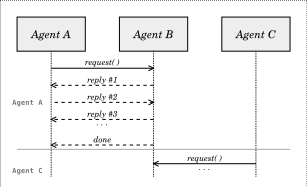
\includegraphics[width=\linewidth]{../figures/executionProblem.pdf}
	\caption{
		Communication with direct method invocation
	}
	\label{fig:direct_method_execution}
\end{figure}
\begin{figure}
	\centering
	\includegraphics[width=\linewidth]{../figures/executionProblem2.pdf}
	\caption{
		Asynchronous commonication
	}
	\label{fig:assynch_execution}
\end{figure}

In \cite{mengistu2008scalability}, authors concluded that increasing the granularity of the system, it is possible to improve its overall performance, even if individual tasks are delayed. The granularity of an agent task is explained as the communication-to-computation, or ``a measure of the amount of computation an agent executes before entering the communication phase of one simulation time step''.

In SAJaS, as in JADE, agent interaction occurs using the messaging service. Therefore, asynchronous execution is appropriate for the kind of applications developed for JADE and SAJaS. Simulations in Repast, though, usually depend on the synchrony of the environment. The use of ACLMessages, which wait in the message queue until processed, allows to maintain a synchronous execution, while simulating an asynchronous one.

To better demonstrate the differences between agent execution in both frameworks, Figures \ref{fig:com-example-repast} and \ref{fig:com-example-jade} represents a scenario where two agents send a message to a third one who then replies. In SAJaS (Fig. \ref{fig:com-example-repast}), messages are delivered to agent C's message queue, and processed only in C's turn. In JADE (Fig. \ref{fig:com-example-jade}), messages can arrive concurrently. Their arrival triggers an event and they are processed right away in the receiving agent's thread. In this case, agent C handles the messages as they arrive and issues the respective replies.

\begin{figure}
	\centering
	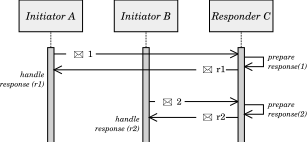
\includegraphics[width=0.9\linewidth]{../figures/tickExample2.pdf}
	\caption{
		Communication in JADE, running in parallel
	}
	\label{fig:com-example-jade}
\end{figure}
\vspace{1cm}
\begin{figure}
	\centering
	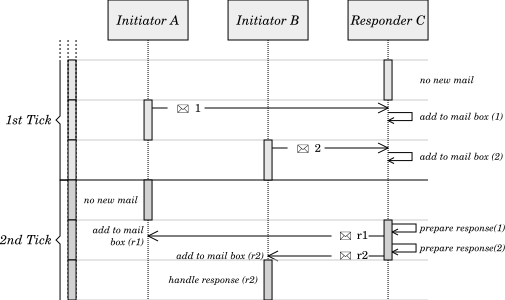
\includegraphics[width=\linewidth]{../figures/tickExample.pdf}
	\caption{
		Communication in SAJaS.
	}
	\label{fig:com-example-repast}
\end{figure}

While the diagram above represents the agents as scheduled objects, their behaviours are the ones actually being scheduled and one agent typically initiates multiple behaviours. It is worth noting that the order by which Repast executes each scheduled behaviour is not predictable. To remove the influence that a fixed execution order can have in the outcome of a simulation, the schedule is randomized every tick. As a result, it is not guaranteed that all the behaviours of a single agent are executed consecutively. This is the expected execution when working with Repast as well as with JADE (given its multi-threaded nature) and it is up to the programmer to ensure that the application does not rely on the order of execution.

\subsection{Messaging issues}
\label{sec:mess_issues}
An issue arose while testing multiple concurrent sessions of agent interaction, as in the case of the second experiment in Section \ref{sec:validation}. The initial implementation of the interaction protocols in SAJaS would receive up to one message from the agent's mail queue in each tick. If the agent would receive N CFPs, then it would take at least N ticks to process them all. While this didn't raise any problem with a single session scenario, with multiple sessions, contract net initiators would start to initiate protocols faster than the responders would terminate them. For this reason, SAJaS was changed so that when possible, all matching ACLMessages should be processed in a single tick.

\subsection{FIPA Specifications}
\label{sec:fipa-specifications}

SAJaS follows JADE architecture very closely, including how FIPA standards are implemented. The implemented features can be divided in the following categories:

\begin{enumerate}
  \item \textbf{Agent Management}, which includes the directory facilitator (DF) service, the structures used by it and the Agent Management Service (AMS),
  \item \textbf{Messaging}, including the ACL Message, the Message Template and the Message Transport Service (MTS), and
  \item \textbf{Interaction Protocols} that allow agents to exchange ACL Messages in a standardized manner; the available protocols are implemented using the classes in Table \ref{tab:fipa_protos}.
\end{enumerate}

\begin{table*}[ht]
	%\normalsize
	\caption{Interaction protocols supported in JADE (adapted from \cite{bellifemine2007developing})}
	\label{tab:fipa_protos}
	\centering
		\begin{tabular}{c|c|c}
			\hline
			\textbf{Protocol(s)} & \textbf{Initiator class} & \textbf{Initiator class} \\
			\hline
			FIPA Request 	& AchieveREInitiator & AchieveREResponder\\
			FIPA Query 		& & \\
			\hline
			FIPA Contract Net & ContractNetInitiator & ContractNetResponder \\
			 &  & SSContractNetResponder \\
			\hline
			FIPA Propose & Propose Initiator & Propose Responder \\
			\hline 
			FIPA Subscribe & SubscriptionInitiator & SubscriptionResponder \\
			\hline
		\end{tabular}
\end{table*}

\section{\uppercase{Code Generation}}
\label{sec:codeconversion}
\noindent There are multiple ways to tackle the problem of code transformations. The brute force approach would be to parse the source code, create an abstract syntax tree (AST), which represents all code constructions in a program, perform certain transformations in the tree, and then generate back the code from the new AST. Fortunately, there are free and open source projects that developers can use to do exactly this with significantly reduced effort.

\subsection{Java Development Tools}
The Eclipse Java Development Tools (JDT)\footnote{https://www.eclipse.org/jdt/} are are a group of tools integrated in the Eclipse IDE. JDT was chosen for the development of the code generation tool. Some of its most interesting features are the automatic cloning of projects, the handling of classes, imports, methods and fields as objects and the possibility of doing complex manipulation tasks without parsing the code. It does, however, allow the use of a high level AST for a more direct manipulation of the source code. JDT is accessible to plugin developers from within Eclipse.

\subsection{MASSim2Dev}
MASSim2Dev is an Eclipse plugin that uses SAJaS. It acts as a translator that, as Figure \ref{fig:conversion_representation} suggests, changes the MABS dependencies from one platform to the equivalent in the other platform. After conversion, no dependency to the previous platform exists in the generated project. Naturally, this is not true for JADE features that are not yet available in SAJaS are used in the MAS. The same happens when using internal features from SAJaS that are not present in JADE.

\begin{figure}[h]
	\centering
	\includegraphics[width=\linewidth]{../figures/conversion_representation.pdf}
	\caption[Representation of the conversion of code]{Representation of the conversion of code.}
	\label{fig:conversion_representation}
\end{figure}

When the plugin is activated, it triggers a series of actions.
\begin{enumerate}
  \item Clone the selected project;
  \item Change all references to SAJaS classes in class imports;
  \item Inject needed libraries in the new project and add them to the build path;
  \item Fix hierarchy (e.g classes that extended \texttt{RepastAgent} must now extend \texttt{Agent}).
\end{enumerate}

When the hierarchy needs to be fixed, it means that the Java type name of the superclass is not the same for JADE and SAJaS. Currently this occurs solely for the Agent class. Throughout SAJaS' code, all references to the agent use the abstract type \texttt{core.Agent}. However, agent types in simulations based on SAJaS+Repast always extend the \texttt{RepastAgent} type.

To perform the mapping of the class imports between the frameworks, a dictionary file exists within the plugin. It allows for quick upgrades to the tool in the future without having to edit the actual code. The dictionary contains annotations that inform how to deal with the hierarchy fixing problem. It also contains information about extra dependencies, such as JADE and Repast libraries.

\section{\uppercase{Validation}}
\label{sec:validation}

\noindent To validate this approach and the developed tools, a set of experiments were designed, in an attempt to cover and test all the available features.

The first example consists of a simple contract net between one buyer and multiple sellers. In the second example, multiple contract nets run concurrently and some of the buyers include available computational trust about sellers. The third example is a board game called Risk developed prior to this project start. The goal of this last example was to test SAJaS with an application that had not been developed specifically for this test, in order do demonstrate that the performance results obtained in generated JADE applications were not caused by faulty code generation.

\subsection{Simple Contract Net}

In this scenario, an agent (the buyer) intends to purchase a certain quantity of goods. It issues a call for proposals (CFP) containing a request for supplies to all agents that announce themselves as suppliers in the DF. After receiving a CFP, the supplier replies with a PROPOSAL containing a price for each product if the demanded supply is within the seller's capacity. Otherwise, a REFUSE message will be sent to the buyer. Finally, the buyer agent compares all valid proposals, chooses the cheapest offer for each of the three products and replies with an ACCEPT PROPOSAL to the best offers, and REJECT PROPOSAL to all others.

To ensure the proper comparison of results, a fixed data set with values for prices and demand was used in both frameworks. This experiment focused on two simple metrics to evaluate the result: time and outcome. After 10 executions, the average performance of the experiment was calculated for each number of agents and is represented in Figure \ref{fig:performance}. The performance of the simulation based on SAJaS was significantly better, excelling when the number of agents is high. JADE was able to perform better when using two distinct containers. The outcome in all executions with the same number of agents was identical.

\input{charts/cnet}

\subsection{Multiple Contract Net}

This scenario is composed by multiple buyers and sellers running simultaneously. After searching the DF for sellers of a given product, each buyer sends the list of sellers to the CTAgent (CT standing for computational trust). The CTAgent keeps track of the sellers' past contracts with buyers and returns the top 5 sellers with the most successful contracts.

With this information, the buyer sends a CFP only to the 5 top agents and accept the best proposal from them. Some sellers will occasionally violate the contract after acceptance. The buyer will then inform the CTAgent if the contract was fulfilled or violated.

Some buyers are programmed to ignore trust and rely solely on the proposal. The premise is that informed buyers eventually avoid contacting sellers programmed to violate contracts more often. The goal of this experiment is to model this scenario in SAJaS, convert it to JADE and verify that the obtained results are very similar.

The experiment was executed 5 times in JADE and 5 times in SAJaS. The scenario is composed of 20 buyers using computational trust, 20 not using trust and 80 sellers. A total of 2000 contracts were recorded to create the following charts in Figures \ref{fig:enterprise_JADE} and \ref{fig:enterprise_SAJaS}. As shown, buyers who made use of computational trust had more successful contracts. The fluctuations early in the simulation are due to the initial lack of trust information. As expected and as shown in the charts, the same outcome was observed both in JADE and SAJaS.

\input{charts/enterprise}

\subsection{RISK board game}

RISK is a multiplayer strategy board game played in turns. It is a game currently owned by Hasbro and the full rules manual is available online \footnote{http://www.hasbro.com/risk/}. The game used for this experiment was developed with JADE before the conception of the project described in this paper. The game is played automatically by agents, competing against each other for the conquest of a map that loosely resembles a world map and its regions. 

Player agents have different behavioural architectures and are classified as aggressive, defensive, opportunistic or random. Communication occurs between the players and the game agent using the FIPA REQUEST protocol. The game also heavily relies on custom Finite State Machine Behaviours (FSMBehaviour) to control game progress. To evaluate the performance of the game, logging features were introduced to the original source code of the application. Other than that, no other changes were made to the original code.

For this experiment, a match with 5 ``random agents'' was setup. Random agents don't follow any particular strategy of attack, defence or soldier distribution and a game with only random agents is always never-ending. To analyse the overall performance of the agent system, the game was converted from JADE to SAJaS. The experiment was then repeated 5 times during 8 seconds and the number of game rounds was registered. The chart in Figure \ref{fig:risk_peformance} shows that SAJaS was capable of executing many more rounds in the same period. The GUI of the game made it possible to assure that the game was executing correctly.

\input{charts/risk}

\section{\uppercase{Conclusions}}
\label{sec:conclusion}

\noindent To bridge the gap between MAS development and simulation, SAJaS was created, allowing JADE developers to create Repast-based simulations using familiar JADE features. MASSim2Dev was also developed to enable the conversion of simulations created with SAJaS into JADE MAS.

Three tests were designed to validate the results of this paper. Technically, the scenarios covered all currently available features in SAJaS. The Achieve RE protocol was used in the Enterprise scenario to communicate with the CT Agent and it was widely used in Risk for all communications. The Contract Net protocol was covered in the first two experiments. The Enterprise scenario also allowed multiple concurrent contracts to take place by using the Responder Dispatcher.

All scenarios made use of the DF service, the AMS, the MTS and of structures like the ACL Message, the Message Template, the DFAgentDescription and the Service Description. The creation of custom Simple Behaviours and Finite State Machine (FSM) Behaviours was covered by Risk. It was possible to demonstrate that bringing JADE and Repast together is not only feasible using the developed tools, but also provides increased performance when compared with JADE MAS.

\section{\uppercase{Future Work}}
\label{sec:futurework}

The proposed system already provides programmers with the means to develop MABS with some complexity. There is, however, still room for development and future enhancements, both to SAJaS and to MASSim2Dv.

\subsection{Increasing SAJaS support of JADE features}
The most immediate extension to this project is to extend the rage of supported JADE features present in SAJaS. While it is important to maintain the simplicity of SAJaS's internals to maintain good simulation performance, more JADE features can be implemented in SAJaS. The core of SAJaS allows to easily extend the API with more interaction protocols and other types of behaviours.

\subsection{Extending native support to other simulation tools}
While developing SAJaS, a conscious effort was made to keep the API very generic, defining a clear separation within SAJaS between Repast-specific elements and everything else. This modularity allows future extensions without changing the API and opens doors to future integration with other simulation tools.

\subsection{Enhancing the plugin with more options and features}
Possible enhancements to the plugin could include providing support for user configurations. From the point of view of the user of the plugin, the code conversion tool provides no flexibility beyond choosing the direction of conversion (from SAJaS to JADE or the reverse). For instance, the plugin could allow the selection of the name and location of the newly generated project, enable the manual selection of the classes to be converted (presently, the whole project is always cloned and transformed) and provide automatic creation of ``stub launchers'' that would allow to quickly test is the generated project executed correctly.

Other configuration options could affect specific internal traits of the generated source code. When a protocol behaviour is expecting messages, one by one all messages that match its template are handled in that tick. The rationale for this design choice was described in Section \ref{sec:mess_issues}. However, the developer may desire to allow only a single message to be processed in each tick. It is still not certain if one approach is the best one in all cases.

\subsection{Enabling support for charts and displays in SAJaS}
One interesting feature in Repast is the ability to create real time visualizations of agent data. This is possible in part because agents in Repast are executed locally, so access to this data is facilitated. In could be interesting to include information display tools - like charts and grids - that could be ported between frameworks. A ``Display Agent'' would handle all visualizations in JADE -- similiar to the sniffer agent -- and agents would provide him with the information to be display.


\vfill
\bibliographystyle{apalike}
{\small
\bibliography{myrefs}}

\vfill
\end{document}

